\documentclass[tikz,border=10pt]{standalone}
\usepackage{amsmath}
\usetikzlibrary{positioning,fit,backgrounds,arrows.meta,decorations.pathreplacing}

% Define node styles
\tikzset{
    mc/.style={rectangle, draw, minimum size=6mm, inner sep=0pt},
    arrow/.style={->, >=Stealth},
    bigarrow/.style={->, >=Stealth, line width=1pt},
}

\begin{document}
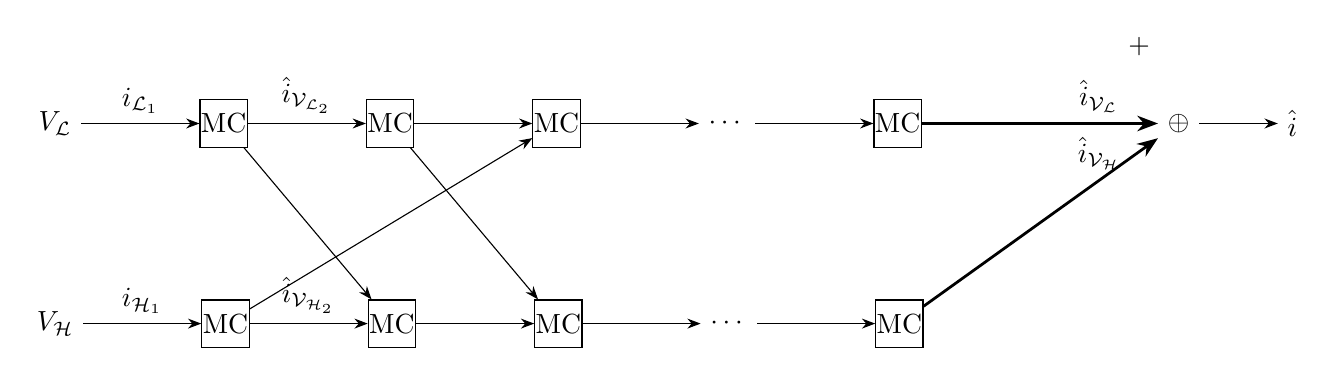
\begin{tikzpicture}[node distance=1.5cm and 1.5cm]

    % Nodes for the top row
    \node (VCL) at (0,0) {$V_{\mathcal{L}}$};
    \node[mc, right=of VCL] (MC1) {MC};
    \node[mc, right=of MC1] (MC2) {MC};
    \node[mc, right=of MC2] (MC3) {MC};
    \node[right=of MC3] (dots1) {$\cdots$};
    \node[mc, right=of dots1] (MC4) {MC};
    
    % Nodes for the bottom row
    \node[below=2cm of VCL] (VHL) {$V_{\mathcal{H}}$};
    \node[mc, right=of VHL] (MC5) {MC};
    \node[mc, right=of MC5] (MC6) {MC};
    \node[mc, right=of MC6] (MC7) {MC};
    \node[right=of MC7] (dots2) {$\cdots$};
    \node[mc, right=of dots2] (MC8) {MC};
    
    % Output nodes
    \node[right=3cm of MC4, label={[xshift=-0.5cm, yshift=0.5cm]$+$}] (plus) {$\oplus$};
    \node[right=1cm of plus] (output) {$\hat{i}$};
    
    % Connections within rows
    \draw[arrow] (VCL) -- (MC1) node[midway, above] {$i_{\mathcal{L}_1}$};
    \draw[arrow] (MC1) -- (MC2) node[midway, above] {$\hat{i}_{\mathcal{V}_{\mathcal{L}_2}}$};
    \draw[arrow] (MC2) -- (MC3);
    \draw[arrow] (MC3) -- (dots1);
    \draw[arrow] (dots1) -- (MC4);
    \draw[bigarrow] (MC4) -- (plus) node[near end, above] {$\hat{i}_{\mathcal{V}_{\mathcal{L}}}$};

    \draw[arrow] (VHL) -- (MC5) node[midway, above] {$i_{\mathcal{H}_1}$};
    \draw[arrow] (MC5) -- (MC6) node[midway, above] {$\hat{i}_{\mathcal{V}_{\mathcal{H}_2}}$};
    \draw[arrow] (MC6) -- (MC7);
    \draw[arrow] (MC7) -- (dots2);
    \draw[arrow] (dots2) -- (MC8);
    \draw[bigarrow] (MC8) -- (plus) node[near end, above] {$\hat{i}_{\mathcal{V}_{\mathcal{H}}}$};

    % Cross connections between rows
    \draw[arrow] (MC1) -- (MC6);
    \draw[arrow] (MC2) -- (MC7);
    \draw[arrow] (MC5) -- (MC3);

    % Final output
    \draw[arrow] (plus) -- (output);
\end{tikzpicture}
\end{document}